\documentclass[main.tex]{subfiles}
 
\begin{document}
\chapterimage{band1.jpg}
\chapter{Security Considerations}

Any discussion about connected devices is incomplete without discussion about the security considerations. Let us look at some of the security considerations that should be taken into account.

\section{Securing Remote Communication}\index{Securing Remote Communication}
All communication with any entity outside of the device must be secured. Instead of reinventing the wheel, we recommend using the standard TLS for securing this communication. The ESP-IDF supports \textit{mbedtls} that implements all the features of the TLS protocol.

All the code in the ESP-Jumpstart already includes this for remote communication. This section is applicable for any other remote connections that you wish to make from your firmware. You can skip to the next section if you are not using any other remote connections.

\subsection{CA Certificates}\index{CA Certificates}
The TLS layer uses trusted CA certificates to validate that the remote endpoint/server is really who it claims to be.

The \textit{esp\_tls} API accepts a CA certificate for performing server validation.

\begin{minted}{c}
        esp_tls_cfg_t cfg = {
            .cacert_pem_buf  = server_root_cert_pem_start,
            .cacert_pem_bytes = server_root_cert_pem_end - server_root_cert_pem_start,
        };

        struct esp_tls *tls = esp_tls_conn_http_new("https://www.example.com", &cfg);
\end{minted}

If this parameter is not present, then the server validation check is skipped. It is strongly recommended that for all your TLS connections you specify the trusted CA certificate that can be used for server validation.

\subsection{Obtaining CA Certificates}\index{Obtaining CA Certificates}
As can be seen from the code above, the trusted CA certificate that can validate your server must be programmed into your firmware. You can obtain the trusted CA certificates by using the following command:

\begin{minted}{bash}
$ openssl s_client -showcerts -connect www.example.com:443 < /dev/null
\end{minted}

This command prints out a list of certificates. The last certificate from this list can be embedded in your device's firmware. Please refer to the Section \ref{sec:embedding_files} for embedding files in your firmware.

\section{Securing Physical Accesses}
Now let us look at some of the features of ESP32 that protect from physically tampering with the device.

\subsection{For ESP8266 Users}\index{For ESP8266 Users}\label{sec:for_esp8266_users}
ESP8266 does not support the following features and thus cannot be secured from physical access.

\subsection{Secure Boot}\index{Secure Boot}
The secure boot support ensures that when the ESP32 executes any software from flash, that software is trusted and signed by a known entity. If even a single bit in the software bootloader and application firmware is modified, the firmware is not trusted, and the device will refuse to execute this untrusted code.

This is achieved by building a chain of trust from the hardware, to the software bootloader to the application firmware.

\begin{figure}[h!]
    \centering
    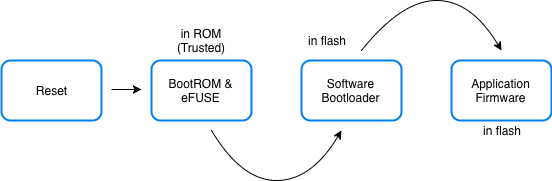
\includegraphics[scale=0.5]{../../_static/secure_boot.png}
    \caption{Secure Boot}
    \label{fig:sec_boot}
\end{figure}

The process works as follows:
\begin{itemize}
\item During manufacturing
  \begin {itemize}
  \item A secret key is programmed into the ESP32's eFUSE. Once programmed this key is protected from software read-out or writes
  \item The software bootloader and the application firmware are signed with the correct keys and the signatures are appended to their images
  \item The signed versions of the bootloader and firmware images are programmed into the ESP32's flash
  \end {itemize}
\item On power on reset of ESP32
  \begin {itemize}
  \item The BootROM uses the secure key in the eFUSE to verify the software bootloader
  \item Once the software bootload is verified, the BootROM loads and executes the software bootloader
  \item The software bootloader verifies the signature of the application firmware
  \item Once the application firmware is verified, the software bootloader loads and executes the application firmware
  \end {itemize}
\end{itemize}

As you might have noticed, you will have to perform some additional steps for enabling secure boot on your devices. Please head over to the detailed information about Secure Boot (\url{https://docs.espressif.com/projects/esp-idf/en/latest/security/secure-boot.html}{Secure Boot}) to understand further.

\subsection{Encrypted Flash}\index{Encrypted Flash}
The flash encryption support ensures that any application firmware, that is stored in the flash of the ESP32, stays encrypted. This allows manufacturers to ship encrypted firmware in their devices.

When flash encryption is enabled, all memory-mapped read accesses to flash are transparently, and at-runtime, decrypted. The flash controller uses the AES key stored in the eFUSE to perform the AES decryption. This encryption key (in the eFUSE) is separate from the secure boot key mentioned above. This key can also be protected from software read-out and writes. Hence only the hardware can perform decryption of the flash contents.

\begin{figure}[h!]
    \centering
    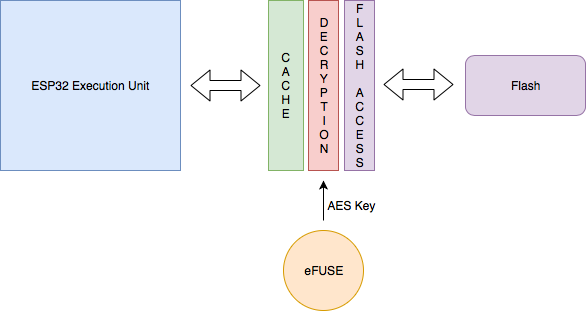
\includegraphics[scale=0.5]{../../_static/flash_encryption.png}
    \caption{Flash Encryption}
    \label{fig:flash_encrypt}
\end{figure}

For more information about enabling flash encryption, you can head over to additional documentation of Flash Encryption (\url{https://docs.espressif.com/projects/esp-idf/en/latest/security/flash-encryption.html}).

\subsection{Encrypting NVS}\index{Encrypting NVS}

The NVS partition has a different access pattern than the application firmware with more frequent writes, and with contents that depend on the user's preferences. Using the same encryption technique that is applicable for application firmware isn't the best option for this scenario. Hence, the ESP-IDF provides a separate encryption mechanism for the NVS partition. This uses the industry-standard AES-XTS encryption that is recommended for protecting data at rest.

The process works as follows:
The process works as follows:
\begin{itemize}
\item During manufacturing
  \begin {itemize}
  \item Create a separate flash partition to store the encryption keys that will be used for NVS encryption
  \item Mark this partition for flash-encryption
  \item Use the \textit{nvs\_partition\_gen.py} tool to generate the partition with random keys
  \item Write this generated partition file into the newly created partition
  \end {itemize}
\item In the firmware
  \begin {itemize}
  \item Call \textit{nvs\_flash\_read\_security\_cfg()} API to read the encryption keys from the above partition and populate them in \textit{nvs\_sec\_cfg\_t}
  \item Initialize the NVS flash partition using the APIs \textit{nvs\_flash\_secure\_init()} or \textit{nvs\_flash\_secure\_init\_partition()}
  \item Perform rest of the NVS operations as you normally would
  \end {itemize}
\end{itemize}

For more information about using NVS encryption, you can head over to the additional documentation at \url{https://docs.espressif.com/projects/esp-idf/en/latest/api-reference/storage/nvs_flash.html#nvs-encryption}.

\end{document}
